\documentclass[11pt,a4paper]{article}

\usepackage[utf8]{inputenc}
\usepackage[T1]{fontenc}
\usepackage[english]{babel}
\usepackage{lmodern}
\usepackage[top=2.5cm,bottom=2.5cm,left=2.7cm,right=2.7cm]{geometry}
\usepackage{amsmath,amssymb,amsthm,mathtools}
\usepackage{graphicx}
\usepackage{booktabs,array}
\usepackage[dvipsnames]{xcolor}
\usepackage{hyperref}
\hypersetup{colorlinks=true,linkcolor=NavyBlue,citecolor=NavyBlue,urlcolor=NavyBlue,
  pdftitle={CTP Core v2.0: reputation with accountable witnesses},pdfauthor={Ange AWALA}}
\usepackage[font=small,labelfont=bf]{caption}

\theoremstyle{plain}
\newtheorem{proposition}{Proposition}
\newtheorem{corollary}{Corollary}
\theoremstyle{definition}
\newtheorem{assumption}{Assumption}
\newtheorem{rulee}{Rule}
\theoremstyle{remark}
\newtheorem{remark}{Remark}

\newcommand{\CTP}{\textsc{ctp}}
\newcommand{\clip}{\operatorname{clip}}
\newcommand{\1}{\mathbf{1}}
\newcommand{\E}{\mathbb{E}}
\newcommand{\Prob}{\mathbb{P}}

\title{\textbf{A Reputation Mechanism with Accountable Witnesses:\\
Model, Calibration and Evaluation of the CommunityTrust Protocol\\(\CTP{} Core v2.0)}}
\author{Ange AWALA\\
\small OpenScience Community --- ORCID 0009-0006-0220-3006\\
\small \texttt{openscience.community@proton.me}}
\date{\small Preprint --- version 2.0 --- not peer reviewed}

\begin{document}
\maketitle

\begin{abstract}
\noindent
Rotating savings groups (tontines) work without formal guarantees because
their members observe each other's past reliability. We study a digital
reputation mechanism inspired by this logic: a member's score evolves with
their contributions, commitment defaults and inactivity, and a contribution
only counts after approval by a randomly drawn panel of \emph{witnesses} who
stake their own score. We correct the model published in v0.1 and v1.1, which
contained demonstrable errors, and derive closed-form conditions for default
tolerance, panel capture by a coalition, profitability of collusion, the
incentive to contribute at maximal score, the verifier's dilemma, and the entry
cost of an identity. These conditions yield a calibration method. Evaluated by
simulation (up to 200 seeds per configuration) against two baselines ---
audit only, and witnesses without accountability ---, with agents that learn to
cheat and to approve without checking, and under a sensitivity analysis, the
recalibrated mechanism makes collusion unprofitable for coalitions of up to
half of the members, whereas audit alone lets $85\,\%$ of frauds through at
the same audit rate. With adaptive agents, it keeps fraud and rubber-stamping at
the exploration level, whereas the v1.1 rules, or removing witness
accountability, lead to collapse (over $90\,\%$ fraud). The sensitivity
analysis revealed two failure modes --- audit errors and small groups ---,
fixed by a counter-audit and an adaptive panel, as well as an applicability
condition: witness accuracy. Finally, we describe an instantiation for
tontines (verifiable payments, score-based rotation order, sponsorship) and a
data collection protocol for its empirical calibration, which remains to be
carried out.

\medskip\noindent
\textbf{Keywords:} reputation systems, tontines, ROSCA, collusion, Sybil
attack, verifier's dilemma, mechanism design, agent-based simulation.
\end{abstract}

% ════════════════════════════════════════════════════════════════
\section{Introduction}
% ════════════════════════════════════════════════════════════════

Rotating savings and credit associations (ROSCAs), called tontines in West
Africa, gather members who periodically pay a contribution whose total is
allocated in turn to one of them~\cite{ardener1964,besley1993,handa1999}. Their
structural weakness is well known: a member who has already received the pot
has an incentive to stop contributing, and enforcement relies on social
pressure and the threat of exclusion~\cite{anderson2009}. Reputation --- the
collective memory of past behaviour --- is therefore the central mechanism.

Digital reputation systems try to reproduce this memory at
scale~\cite{resnick2000,dellarocas2003,josang2007}. They face well-documented
difficulties: manipulation by coalitions, multiple identities (Sybil
attack~\cite{douceur2002}), reputation laundering through identity
change~\cite{friedman2001}, and verifier laziness when checking is
costly~\cite{luu2015}.

The CommunityTrust Protocol (\CTP{}) proposes a mechanism in which a
contribution only counts after approval by \emph{witnesses} who risk their own
score. Versions v0.1 and v1.1 claimed universality and strategic robustness; a
review showed that these claims were not established
(Appendix~\ref{app:erratum}).

\paragraph{Contributions.}
\begin{enumerate}
  \item A consistent formal model with explicit assumptions
    (Section~\ref{sec:model}).
  \item Nine propositions and two corollaries, including seven closed-form
    conditions usable for calibration (Section~\ref{sec:analysis}).
  \item A parameter set derived from these conditions
    (Section~\ref{sec:calibration}).
  \item A reproducible simulation study: verification of the conditions,
    comparison with two baselines, adaptive agents and sensitivity analysis
    (Section~\ref{sec:simulation}).
  \item An instantiation for tontines with two results on rotation order and
    sponsorship (Section~\ref{sec:tontine}).
  \item An erratum of the previous versions and a data collection protocol
    (Appendices~\ref{app:erratum} and~\ref{app:data}).
\end{enumerate}

\paragraph{What this paper does not claim.} The idea of a continuous, dynamic,
non-transferable trust score is not new (Section~\ref{sec:related}). The
results concern a model; no field data is used yet. The Node hierarchy, global
score and portability of previous versions are out of scope
(Appendix~\ref{app:extensions}).

% ════════════════════════════════════════════════════════════════
\section{Related work}
\label{sec:related}
% ════════════════════════════════════════════════════════════════

\paragraph{Computational trust and reputation.} Marsh~\cite{marsh1994}
formalises trust as a continuous quantity updated by experience. Resnick et
al.~\cite{resnick2000}, Dellarocas~\cite{dellarocas2003} and Jøsang et
al.~\cite{josang2007} describe rating-based mechanisms and their failure modes.
EigenTrust~\cite{kamvar2003} aggregates local ratings into a global score;
PeerTrust~\cite{xiong2004} weights feedback by the credibility of its source ---
a principle \CTP{} reuses by weighting a contribution's quality by the score of
its approvers.

\paragraph{Attacks.} Without an authority certifying identities, an attacker
can always present multiple identities~\cite{douceur2002}, and no symmetric
reputation function is robust to this~\cite{cheng2005}. When pseudonyms are
free, newcomers must start at the minimal score, otherwise identity change
erases sanctions~\cite{friedman2001}. Hoffman et al.~\cite{hoffman2009} survey
these attacks and their defences.

\paragraph{Incentivised verification.} Luu et al.~\cite{luu2015} describe the
\emph{verifier's dilemma}: when checking is costly and fraud is rare, a
rational verifier accepts without checking. TrueBit~\cite{teutsch2017}
addresses it by injecting deliberate errors (\emph{forced errors}) that
verifiers are rewarded for detecting. Kleros~\cite{kleros2019} draws jurors at
random who post a deposit and are rewarded when voting with the majority.
\CTP{} combines these ideas: random panel, majority reward, score-proportional
sanction, decoy signals.

\paragraph{Repeated games and community norms.} Sustaining cooperation through
the threat of future sanctions falls under the folk theorem~\cite{fudenberg1986};
Kandori~\cite{kandori1992} studies sanctions exercised by the community. The
``dominance'' conditions of v1.1 were instances of these results and are not
claimed as contributions.

\paragraph{Tontines and joint liability.} Besley, Coate and
Loury~\cite{besley1993} and Handa and Kirton~\cite{handa1999} analyse the
economics of ROSCAs; Anderson, Baland and Moene~\cite{anderson2009} study
enforcement after the pot has been received. Abebe et al.~\cite{abebe2022}
study ROSCAs from an algorithmic perspective. Joint liability in
microcredit~\cite{besley1995,ghatak1999} underpins the sponsorship mechanism of
Section~\ref{sec:tontine}. Ostrom~\cite{ostrom1990} studies the governance of
commons without an external authority.

\paragraph{Non-transferable reputation.} Critiques of token-weighted
voting~\cite{buterin2021} and non-transferable tokens~\cite{weyl2022} share the
goal of decoupling influence from wealth.

% ════════════════════════════════════════════════════════════════
\section{Model}
\label{sec:model}
% ════════════════════════════════════════════════════════════════

\subsection{Agents, periods and signals}

A Node (community) has $n$ members. Time is discrete, $t\in\mathbb{N}$. Each
member $i$ has a score $\tau_i(t)\in[0,1]$. In each period, a member either
\emph{defaults} on their commitment, submits a signal $s$ (candidate
contribution), or does nothing. Each signal has a true conformity
$Q(s)\in\{0,1\}$ that the protocol does not observe directly.

\subsection{Witness panel and acceptance}

A member is eligible as a witness if $\tau_w(t)\ge\tau_W$. For each signal, a
panel $\mathcal{P}(s)$ of $k$ witnesses is drawn uniformly without replacement
among eligible members other than the author, with
$k=\max(k_{\min},\lfloor\alpha_k(n-1)\rfloor)$. Each witness approves or
rejects; $\mathcal{A}(s)$ denotes the approvers. The signal is accepted if
$|\mathcal{A}(s)|\ge a_k=\lceil\theta k\rceil$. If fewer than $k$ members are
eligible, the panel is reduced to all $m$ eligible members when $m\ge3$ (with
$a_m=\lceil\theta m\rceil$); if $m<3$, the signal is provisionally accepted and
audited with certainty. Without this rule, a small Node in which a few members
fall below $\tau_W$ can no longer evaluate any signal
(Section~\ref{sec:simulation}, E7). The measured quality of an accepted signal
is
\begin{equation}
q(s)=\bar\tau_{\mathcal{A}(s)}\cdot\frac{|\mathcal{A}(s)|}{k}.
\label{eq:q}
\end{equation}

\subsection{Audit and decoy signals}

Each accepted contribution is independently audited with probability $p_a$; the
audit reveals $Q(s)$ with error probability $\varepsilon_a$. A non-conformity
verdict triggers an independent \emph{counter-audit}; the contribution is
\emph{sanctioned} only if both verdicts agree. The probability of sanctioning a
conforming contribution thus drops from $\varepsilon_a$ to $\varepsilon_a^2$,
at the cost of letting an audited non-conforming contribution through with
probability at most $2\varepsilon_a$. In addition, in each period and for each
member, the protocol injects a \emph{decoy signal} with probability $h$: a
signal known to be non-conforming, presented to a panel like an ordinary one.

\subsection{Score dynamics}

\begin{equation}
\boxed{\tau_i(t+1)=\clip\bigl(\tau_i+G_i+R_i-L_i-S_i-D_i-W_i,\;0,\;1\bigr)}
\label{eq:dyn}
\end{equation}
\begin{align}
G_i&=\eta\textstyle\sum_{s\,:\,\text{author}=i,\ \text{accepted, not sanctioned}}q(s)
  &&\text{author gain}\label{eq:G}\\
R_i&=\tfrac{\eta_W}{k}\cdot\#\{s: i\in\mathcal{P}(s),\ \text{vote of } i=\text{outcome of } s\}
  &&\text{majority reward}\label{eq:R}\\
L_i&=\kappa\,\1\{i\text{ defaults}\}&&\text{commitment default}\label{eq:L}\\
S_i&=\kappa_s\cdot\#\{s:\text{author}=i,\ \text{sanctioned}\}&&\text{author sanction}\label{eq:S}\\
D_i&=\delta\,\tau_i\,\1\{i\text{ inactive}\}&&\text{depreciation}\label{eq:D}\\
W_i&=\phi\,\tau_i\cdot\#\{s: i\in\mathcal{A}(s),\ s\text{ sanctioned or decoy}\}
  &&\text{witness accountability}\label{eq:W}
\end{align}
The \emph{outcome} of a signal is either ``accepted and not sanctioned'' or
``rejected or sanctioned''; a decoy always has the latter outcome. A member is
\emph{inactive} if they have neither an accepted, non-sanctioned contribution
nor a default in the period: submitting a rejected signal is not enough to
remain active. The reward $R_i$ is only paid to a member who is active in the
period: it cannot compensate for not contributing.

\paragraph{Differences from v1.1 and rationale.} (i) $R_i$ is new: without it,
validating brings nothing and carries a risk. It rewards agreement with the
outcome rather than approval, so as not to bias votes towards approval.
(ii) $S_i$ is new: without it, submitting a fraud is riskless. (iii) The
witness sanction is no longer divided by $|\mathcal{A}(s)|$: the division
diluted accountability as accomplices became more numerous. (iv) Auditing is
uniform instead of being restricted to signals with low $q(s)$.
(v) Inactivity is defined by the absence of an accepted contribution.
(vi) Decoy signals are new (Prop.~\ref{prop:verif}). (vii) The witness reward
is conditional on activity: without this rule, a member who never contributes
could keep their score by serving only as a witness (observed in simulation:
stationary score of about $0.3$ for free riders). (viii) The counter-audit and
panel reduction are new; both fix failures observed in simulation (E7).

\subsection{Assumptions}

\begin{assumption}[Audit]\label{h:audit}
An audit reveals the true conformity, with error probability $\varepsilon_a$
(zero unless stated otherwise).
\end{assumption}
\begin{assumption}[Non-manipulable draw]\label{h:draw}
The panel is drawn uniformly; neither the author nor the witnesses choose it,
and decoy signals are indistinguishable from ordinary ones.
\end{assumption}
\begin{assumption}[Entry]\label{h:entry}
Founding members start at $\tau_0$; every newcomer starts at 0, unless
sponsored (Section~\ref{sec:tontine}).
\end{assumption}
\begin{assumption}[Utility]\label{h:lin}
For the strategic analysis, utility is linear in score, away from the bounds,
minus effort costs: $c_h$ for a conforming contribution, $c_v$ for a check.
\end{assumption}

% ════════════════════════════════════════════════════════════════
\section{Analysis}
\label{sec:analysis}
% ════════════════════════════════════════════════════════════════

\begin{proposition}[Boundedness]
If $\tau_i(0)\in[0,1]$ for all $i$, then $\tau_i(t)\in[0,1]$ for all $t$.
\end{proposition}
\begin{proof}
By induction, since $\clip$ takes values in $[0,1]$.
\end{proof}

\begin{proposition}[Saturation]\label{prop:sat}
If a member obtains in every period an accepted, non-sanctioned contribution of
quality $q(s)\ge\underline q>0$, with no negative term, then $\tau_i(t)=1$ for
all $t\ge\lceil(1-\tau_i(0))/(\eta\underline q)\rceil$.
\end{proposition}
\begin{proof}
Each period adds at least $\eta\underline q$ as long as $\tau_i<1$.
\end{proof}

\begin{proposition}[Decay under inactivity]
A member inactive over $[0,t]$ satisfies $\tau_i(t)=\tau_i(0)(1-\delta)^t$.
\end{proposition}

\subsection{Default tolerance}

\begin{proposition}[Tolerance threshold]\label{prop:default}
Consider a member who defaults with probability $p_d$ per period and otherwise
obtains an accepted, conforming contribution of mean quality $\bar q$. For
$\tau_i\in[\kappa,1-\eta]$, $\E[\Delta\tau_i]=(1-p_d)\eta\bar q-p_d\kappa$,
which is strictly positive if and only if
\begin{equation}
p_d<p^\star_d=\frac{\eta\bar q}{\eta\bar q+\kappa}.
\label{eq:pstar}
\end{equation}
\end{proposition}
\begin{proof}
In this interval no bound is reached within one period; default and
contribution are mutually exclusive; take expectations.
\end{proof}

\begin{corollary}[Calibrating $\kappa$]\label{cor:kappa}
For a target tolerance $p^\star$, one needs
$\kappa=\eta\bar q\,(1-p^\star)/p^\star$: the ratio $\kappa/\eta$, not the
absolute values, sets the tolerance.
\end{corollary}

\subsection{Panel capture}

\begin{proposition}[Capture probability]\label{prop:capture}
Let there be $m$ eligible members other than the author, including $c$
accomplices who unconditionally approve the coalition's signals, the others
rejecting non-conforming signals. The probability that a non-conforming
coalition signal is accepted is at least
\begin{equation}
\pi(m,c,k,a_k)=\sum_{x=a_k}^{\min(c,k)}
\frac{\binom{c}{x}\binom{m-c}{k-x}}{\binom{m}{k}},
\label{eq:hyper}
\end{equation}
with equality if honest witnesses never err.
\end{proposition}
\begin{proof}
Under Assumption~\ref{h:draw}, the number of accomplices in the panel follows a
hypergeometric distribution $(m,c,k)$; honest witnesses' errors can only add
approvals.
\end{proof}

\subsection{Profitability of collusion}

\begin{proposition}[Audit threshold]\label{prop:collusion}
Consider a non-conforming coalition contribution, accepted with quality $q$ by
$x\ge a_k$ accomplices of mean score $\bar\tau$. The coalition's expected gain
is $\E[\Delta]=(1-p_a)(\eta q+x\eta_W/k)-p_a(\kappa_s+\phi x\bar\tau)$, which is
negative if and only if
\begin{equation}
p_a>p^\star_a=\frac{\eta q+x\eta_W/k}{\eta q+x\eta_W/k+\kappa_s+\phi x\bar\tau}.
\label{eq:pa}
\end{equation}
Since $q\le1$, $x\eta_W/k\le\eta_W$, $x\ge a_k$ and $\bar\tau\ge\tau_W$,
$p^\star_a\le(\eta+\eta_W)/(\eta+\eta_W+\kappa_s+\phi a_k\tau_W)$.
\end{proposition}
\begin{proof}
If not sanctioned, the contribution yields $\eta q$ to the author and
$\eta_W/k$ to each approving accomplice; if sanctioned, it costs $\kappa_s$ to
the author and $\phi\tau_w$ to each approver. The bound follows from the
monotonicity of $p^\star_a$ in each term.
\end{proof}

\begin{corollary}[Collusion without audit]\label{cor:noaudit}
Assume $p_a=0$ and a homogeneous coalition with score $\tau$, each of whose
non-conforming signals is accepted with probability $\pi$ and rejected
otherwise. If inactivity is defined by the absence of an accepted contribution,
the expected per-period score change of a colluder is at most
$\pi\eta\tau-(1-\pi)\delta\tau$ (away from the bounds, excluding witness
rewards), which is negative as soon as
\begin{equation}
\frac{\pi}{1-\pi}<\frac{\delta}{\eta}.
\label{eq:noaudit}
\end{equation}
With $\delta=\eta$, collusion only pays if the coalition captures more than
half of the panels. If inactivity is defined by the absence of submission
(v1.1 rule), a rejected signal costs nothing and collusion pays for any
$\pi>0$.
\end{corollary}
\begin{proof}
If accepted (probability $\pi$), the signal yields $\eta q\le\eta\tau$ since
$q=\bar\tau_{\mathcal{A}}|\mathcal{A}|/k\le\tau$ for approvers with score
$\tau$; if rejected, the colluder is inactive and loses $\delta\tau$.
\end{proof}

Proposition~\ref{prop:collusion} remains necessary when $\pi$ exceeds this
threshold --- a majority coalition --- or when depreciation is small relative to
the gain.

\subsection{Incentive at maximal score}

\begin{proposition}[Ceiling]\label{prop:ceiling}
A member at score $\tau_i=1$ gains nothing from an accepted contribution. Under
Assumption~\ref{h:lin}, contributing honestly is better than submitting a
non-conforming signal (rejected with probability $1-\pi_1$) if
\begin{equation}
c_h<(1-\pi_1)\,\delta+\pi_1\,p_a\,\kappa_s,
\label{eq:ceiling}
\end{equation}
where $\pi_1$ is the probability that an isolated non-conforming signal is
accepted. If inactivity is defined by the absence of \emph{submission} (v1.1
rule), a saturated member is never inactive, the right-hand side reduces to
$\pi_1 p_a\kappa_s$, and honest contribution is no longer incentivised once
$c_h>\pi_1p_a\kappa_s$.
\end{proposition}
\begin{proof}
At $\tau_i=1$, $G_i$ is absorbed by the ceiling. An honest contribution costs
$c_h$ and avoids depreciation $\delta$. A non-conforming signal costs nothing;
if rejected (probability $1-\pi_1$) it leaves the member inactive (loss
$\delta$); if accepted it avoids depreciation but exposes the member to the
sanction $\kappa_s$ with probability $p_a$.
\end{proof}

\subsection{Verifier's dilemma}

\begin{proposition}[Decoy signals]\label{prop:verif}
A witness with score $\tau_w$ can \emph{check} (cost $c_v$) or
\emph{rubber-stamp} (approve without checking). Let $h'$ be the share of decoy
signals among the signals presented. Counting decoys only, rubber-stamping is
strictly dominated if
\begin{equation}
h'\,\bigl(\phi\,\tau_w+\eta_W/k\bigr)>c_v.
\label{eq:verif}
\end{equation}
Without decoys ($h'=0$) and if real frauds are rare, rubber-stamping is the
best response: this is the verifier's dilemma.
\end{proposition}
\begin{proof}
On a conforming signal, checking and rubber-stamping lead to the same vote
(approval) and the same reward; only $c_v$ differs. On a decoy,
rubber-stamping costs $\phi\tau_w$ and forfeits $\eta_W/k$, whereas checking
leads to rejection (barring error). Real non-conforming signals only add to the
advantage of checking.
\end{proof}

\subsection{Entry cost}

\begin{proposition}[Eligibility delay]\label{prop:sybil}
Under Assumption~\ref{h:entry}, a new unsponsored identity cannot be a witness
before $\lceil\tau_W/\eta\rceil$ periods, each including an accepted
contribution.
\end{proposition}
\begin{proof}
A non-witness member gains at most $\eta q\le\eta$ per period, and nothing
without an accepted contribution.
\end{proof}

The mechanism therefore does not make Sybil attacks impossible --- which is ruled
out for a symmetric function~\cite{cheng2005} --- but gives them a cost linear in
the number of identities, which is deterrent only if an accepted contribution
is itself costly. Since the score is bounded below by 0, the effective sanction
of a default is $\min(\kappa,\tau_i)$; Section~\ref{sec:tontine} addresses this
limit through exclusion and sponsorship.

% ════════════════════════════════════════════════════════════════
\section{Calibration}
\label{sec:calibration}
% ════════════════════════════════════════════════════════════════

Table~\ref{tab:params} derives the recommended parameters (v2.1) from the
propositions above. The v1.1 parameters, kept for comparison, are labelled v2.0
when used with the corrected model.

\begin{table}[h]
\centering
\caption{Parameters: original v1.1 and recommended v2.1.}
\label{tab:params}
\small
\begin{tabular}{clccl}
\toprule
& Role & v1.1 & v2.1 & Rationale for v2.1 \\
\midrule
$\eta$ & author gain & $0.05$ & $0.02$ & saturation in $\approx55$ periods (Prop.~\ref{prop:sat}) \\
$\kappa$ & default penalty & $0.15$ & $0.35$ & $p^\star_d\approx0.05$ (Cor.~\ref{cor:kappa}) \\
$\eta_W$ & witness reward & --- & $0.005$ & small relative to $\eta$ \\
$\kappa_s$ & author sanction & --- & $0.10$ & \\
$\phi$ & witness accountability & $0.15$ & $0.30$ & $p^\star_a\le0.052$ (Prop.~\ref{prop:collusion}) \\
$p_a$ & audit probability & $0.15$ & $0.15$ & $\approx3\times$ margin over $p^\star_a$ \\
$k_{\min}$ & minimal panel size & $3$ & $5$ & $\pi\approx0.006$ for 30\,\% accomplices, $n=20$ \\
$\theta$ & approval fraction & $1$ & $2/3$ & tolerance to witness errors \\
$h$ & decoy rate & --- & $0.05$ & $h'\approx0.048>0.011$ (Prop.~\ref{prop:verif}) \\
$\delta$ & depreciation & $0.02$ & $0.02$ & $>c_h$ required (Prop.~\ref{prop:ceiling}) \\
$\alpha_k$ & panel fraction & $0.20$ & $0.20$ & \\
$\tau_W$ & eligibility threshold & $0.30$ & $0.30$ & \\
$\tau_0$ & founders' score & --- & $0.50$ & choice (sensitivity in E7) \\
\bottomrule
\end{tabular}
\end{table}

Two parameter-free rules are added: the counter-audit and the adaptive panel
(Section~\ref{sec:model}). The numerical rationales use $\bar q=0.91$ (measured
in simulation) and, for Proposition~\ref{prop:verif}, $c_v=0.001$ and
$\tau_w=\tau_W$. For the v1.1 parameters, the same
Proposition~\ref{prop:default} gives $p^\star_d=0.23$: a member can default
about one period in four while seeing their score increase.

% ════════════════════════════════════════════════════════════════
\section{Simulation study}
\label{sec:simulation}
% ════════════════════════════════════════════════════════════════

\subsection{Protocol}

The simulations implement exactly the model of Section~\ref{sec:model} over
$T=104$ periods (300 for E6). 95\,\% confidence intervals are obtained by
bootstrap over seeds. Behaviours: \emph{honest} (true quality
$\sim\mathcal N(0.72;0.12)$); \emph{free rider} (active with probability
$0.08$, quality $\sim\mathcal U(0.10;0.35)$); \emph{isolated fraudster}
(quality $\sim\mathcal N(0.20;0.08)$, honest witness); \emph{colluder} (like the
fraudster, but unconditionally approves other colluders' signals);
\emph{adaptive} (E6). A signal is conforming if its true quality is at least
$0.45$; a checking witness observes it with noise
$\mathcal N(0;\sigma_{\text{obs}})$, $\sigma_{\text{obs}}=0.10$. Three rule sets
are compared: \textbf{v1.1} (original rules and parameters), \textbf{v2.0}
(corrected model, v1.1 parameters, no decoys, divided sanction, inactivity
defined by absence of submission), \textbf{v2.1} (corrected model,
Table~\ref{tab:params} parameters).

\subsection{E1 --- Default tolerance}

Twenty honest members, five of whom default with probability $p_d$
(Figure~\ref{fig:E1}).

\begin{figure}[h]
\centering
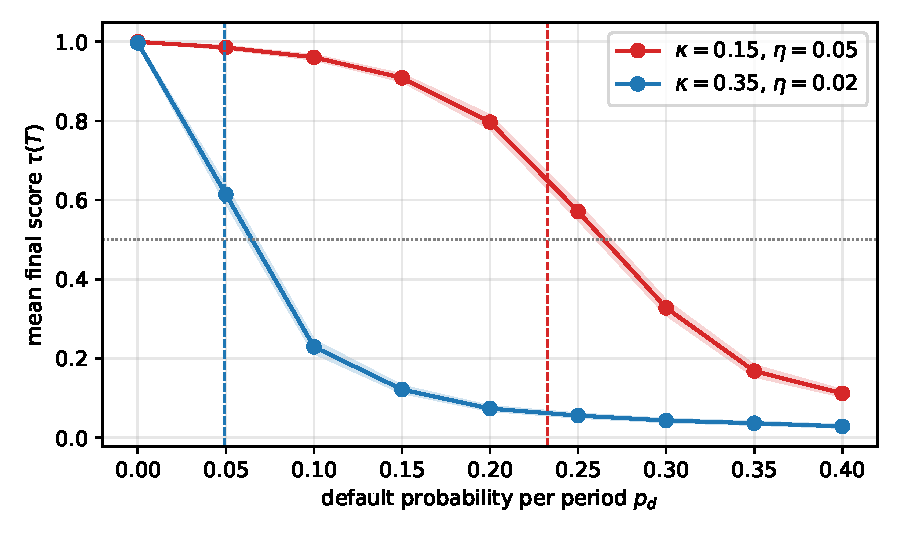
\includegraphics[width=0.7\textwidth]{figures/fig_E1_defaut_en.pdf}
\caption{E1 --- Final score of defaulting members (95\,\% CI, 200 seeds).
Dashed: threshold $p^\star_d$ (Prop.~\ref{prop:default}); dotted: initial score.}
\label{fig:E1}
\end{figure}

With the v1.1 parameters ($p^\star_d=0.23$), members defaulting one period in
seven end at $0.91$ $[0.90;0.92]$, and the final score only drops below the
initial score between $p_d=0.25$ and $p_d=0.30$. With the v2.1 parameters
($p^\star_d=0.049$), defaulting one period in twenty leaves the score at
$0.61$ $[0.60;0.63]$, slightly above the initial score as expected near the
threshold, and defaulting one period in ten brings it down to $0.23$
$[0.22;0.25]$. Both observed thresholds agree with (\ref{eq:pstar}) up to the
offset due to the variation of $\bar q$ and to the bounds.

\subsection{E2 --- Collusion and audit probability}

Coalitions of 8 and 12 members out of 20 (40\,\% and 60\,\%)
(Figure~\ref{fig:E2}).

\begin{figure}[h]
\centering
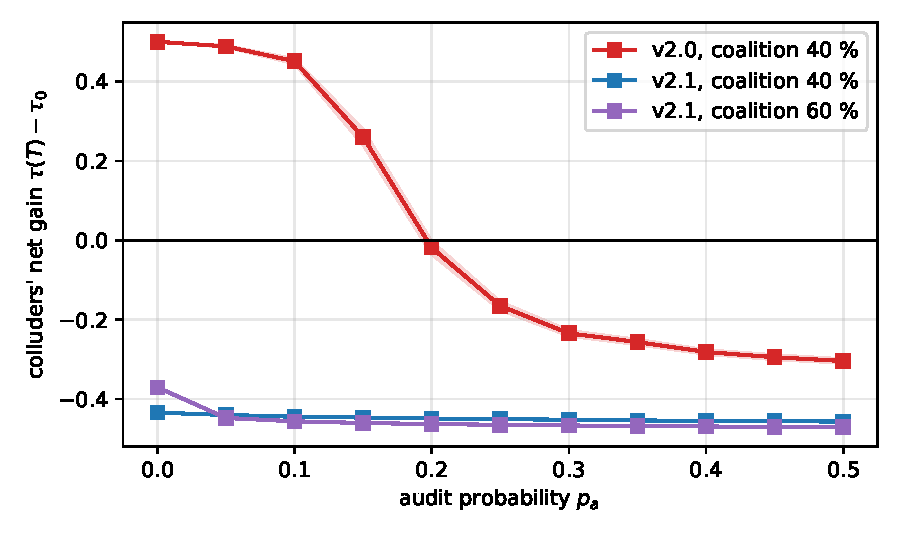
\includegraphics[width=0.7\textwidth]{figures/fig_E2_collusion_en.pdf}
\caption{E2 --- Mean net gain of a coalition as a function of $p_a$ (95\,\% CI, 200 seeds).}
\label{fig:E2}
\end{figure}

With the v1.1 parameters (40\,\% coalition), the net gain is $+0.50$ without
audit, $+0.26$ $[0.24;0.28]$ at $p_a=0.15$, no longer significantly non-zero
at $p_a=0.20$ ($-0.02$ $[-0.04;0.00]$), and negative beyond, in line with the
threshold of Proposition~\ref{prop:collusion} in its divided-sanction form
($0.146$ to $0.194$). With v2.1, collusion loses \emph{for every value of
$p_a$, including zero}: $-0.43$ without audit for a 40\,\% coalition and $-0.37$
for a 60\,\% coalition. This is what Corollary~\ref{cor:noaudit} predicts:
with $\delta/\eta=1$, collusion requires $\pi>1/2$, whereas the capture
probability is about $0.04$ at 40\,\% (E3) and $\pi(19,11,5,4)\approx0.27$ at
60\,\%. In v2.1, it is the inactivity rule, not the audit, that deters
minority collusion; the audit remains the protection against a majority
coalition and against careless witnesses (E6).

\subsection{E3 --- Panel capture}

Acceptance rate of a coalition's non-conforming signals, $n=20$, no audit
(Figure~\ref{fig:E3}).

\begin{figure}[h]
\centering
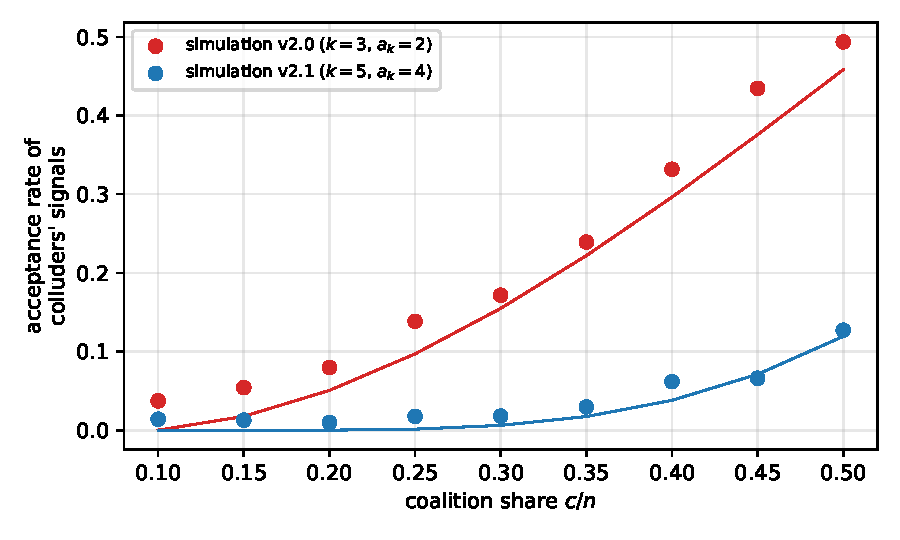
\includegraphics[width=0.7\textwidth]{figures/fig_E3_capture_en.pdf}
\caption{E3 --- Dots: simulation (100 seeds); lines: hypergeometric bound of
Proposition~\ref{prop:capture}.}
\label{fig:E3}
\end{figure}

With the v1.1 parameters ($k=3$, $a_k=2$), a 30\,\% coalition gets $17\,\%$ of
its non-conforming signals accepted, and a half-size coalition $49\,\%$. With
v2.1 ($k=5$, $a_k=4$), these rates drop to $1.8\,\%$ and $12.7\,\%$. Measured
rates exceed the bound (\ref{eq:hyper}) by the effect of honest witnesses'
errors, up to sampling noise (45\,\%).

\subsection{E4 --- Comparison of the three rule sets}

Twenty members: 10 honest ($p_d=0.02$), 4 free riders, 6 colluders
(Table~\ref{tab:E4}, Figure~\ref{fig:E4}).

\begin{table}[h]
\centering
\caption{E4 --- Mean final score per group and error rates (200 seeds; 95\,\% CI in brackets).}
\label{tab:E4}
\small
\begin{tabular}{lccc}
\toprule
& v1.1 & v2.0 & v2.1 \\
\midrule
Honest & $0.99$ $[0.99;0.99]$ & $0.99$ $[0.99;0.99]$ & $0.91$ $[0.91;0.92]$ \\
Free riders & $0.07$ $[0.07;0.07]$ & $0.07$ $[0.07;0.07]$ & $0.06$ $[0.06;0.06]$ \\
Colluders & $0.58$ $[0.57;0.58]$ & $0.78$ $[0.77;0.80]$ & $0.06$ $[0.06;0.06]$ \\
\midrule
Frauds accepted & $2.5\,\%$ & $19.1\,\%$ & $0.5\,\%$ \\
Wrongful rejections & $8.6\,\%$ & $1.6\,\%$ & $3.7\,\%$ \\
Votes per signal & $3.0$ & $3.0$ & $5.3$ \\
Audits per signal & $0.00$ & $0.10$ & $0.09$ \\
\bottomrule
\end{tabular}
\end{table}

\begin{figure}[h]
\centering
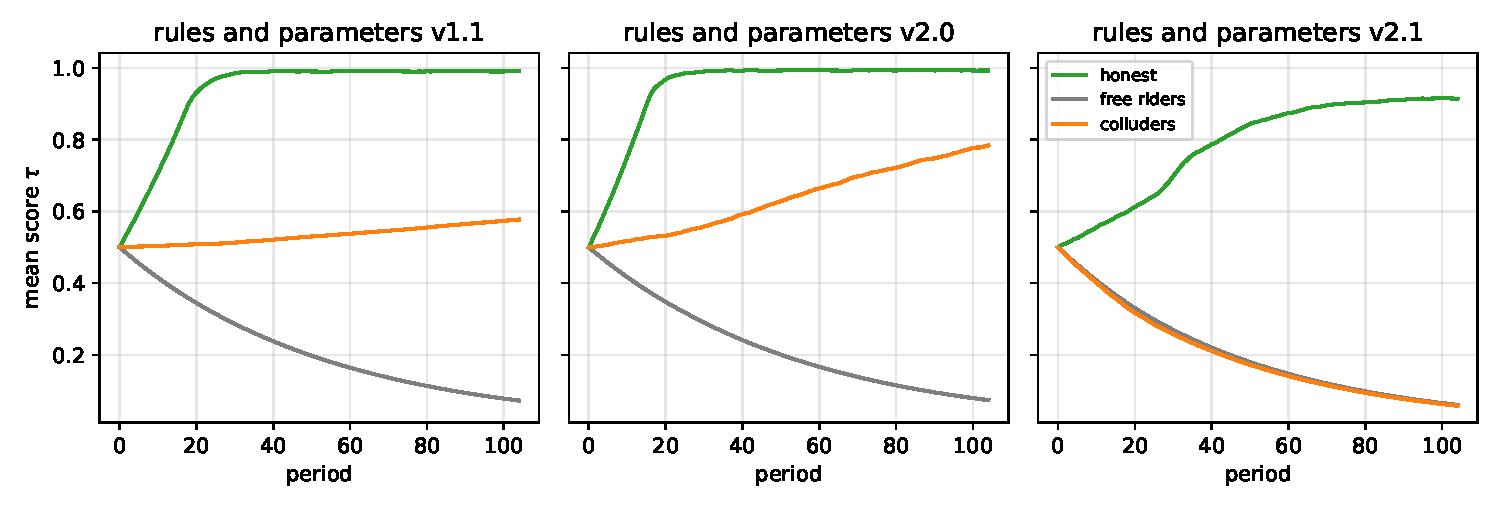
\includegraphics[width=\textwidth]{figures/fig_E4_comparaison_en.pdf}
\caption{E4 --- Mean score trajectories per group.}
\label{fig:E4}
\end{figure}

With v1.1, colluders end above their initial score ($0.58$): their rare
captured contributions have $q(s)$ above $q_{\min}$ and are never audited, and
unanimity wrongly rejects $8.6\,\%$ of honest contributions. The corrected
model with v1.1 parameters (v2.0) is \emph{worse}: $19\,\%$ of frauds are
accepted and colluders reach $0.78$, because 2-out-of-3 approval multiplies the
capture probability by fifteen ($\pi\approx0.010\to0.155$), $p_a$ stays below
threshold, and a rejected signal costs nothing. With v2.1, colluders fall to
the free riders' level ($0.06$) and $0.5\,\%$ of frauds pass. The trade-off is a
mean honest score of $0.91$ instead of $0.99$: a harsher default penalty and
$3.7\,\%$ wrongful rejections make accidental defaults ($p_d=0.02$) costly. This
cost follows directly from the choice of $p^\star_d$ and can be tuned via
Corollary~\ref{cor:kappa}.

\subsection{E5 --- Do witnesses add anything?}

To isolate the contribution of witnesses, v2.1 is compared with two baselines at
the same $p_a=0.15$: \emph{audit only} (every contribution is accepted with
$q=1$, and only the audit sanctions) and \emph{witnesses without accountability}
($\phi=\kappa_s=\eta_W=h=0$). Population: 13 honest members, 3 isolated
fraudsters, 4 colluders (Table~\ref{tab:E5}).

\begin{table}[h]
\centering
\caption{E5 --- Comparison with baselines (200 seeds).}
\label{tab:E5}
\small
\begin{tabular}{lccc}
\toprule
& audit only & no accountability & v2.1 \\
\midrule
Honest & $1.00$ $[1.00;1.00]$ & $1.00$ $[1.00;1.00]$ & $1.00$ $[1.00;1.00]$ \\
Isolated fraudsters & $0.52$ $[0.50;0.54]$ & $0.06$ $[0.06;0.06]$ & $0.06$ $[0.06;0.06]$ \\
Colluders & $0.53$ $[0.51;0.55]$ & $0.06$ $[0.06;0.06]$ & $0.06$ $[0.06;0.06]$ \\
\midrule
Frauds accepted & $84.9\,\%$ & $0.2\,\%$ & $0.2\,\%$ \\
Wrongful rejections & $0.0\,\%$ & $3.8\,\%$ & $3.7\,\%$ \\
Votes per signal & $0.0$ & $5.0$ & $5.2$ \\
Audits per signal & $0.15$ & $0.09$ & $0.09$ \\
\bottomrule
\end{tabular}
\end{table}

\begin{figure}[h]
\centering
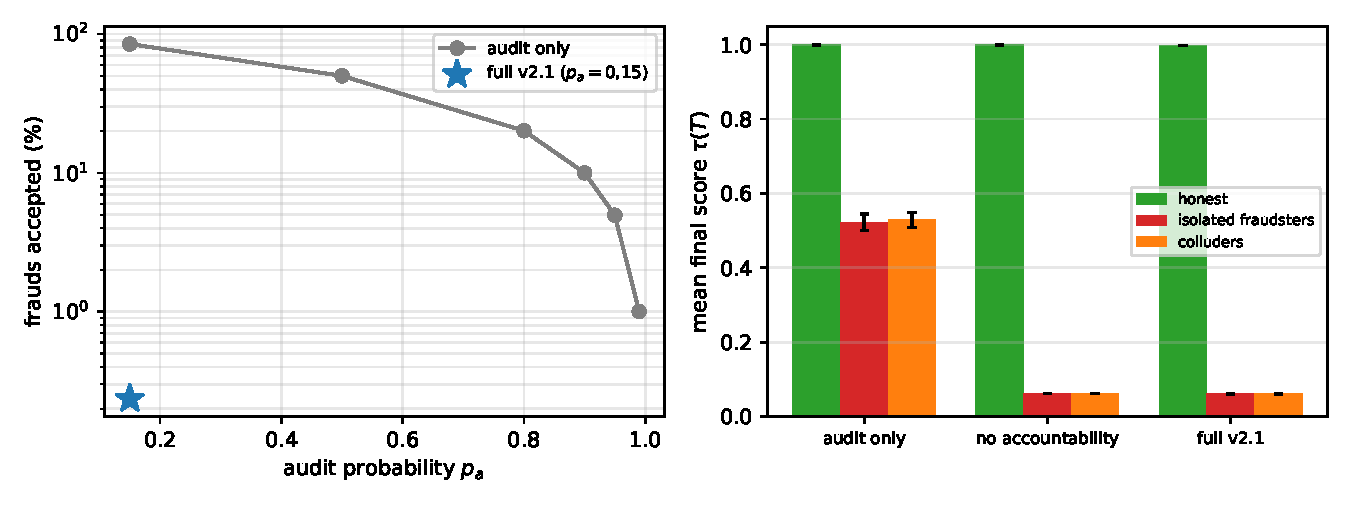
\includegraphics[width=0.95\textwidth]{figures/fig_E5_references_en.pdf}
\caption{E5 --- Left: share of frauds accepted by audit alone as a function of
$p_a$ (log scale), compared with v2.1 at $p_a=0.15$. Right: final score per
group (95\,\% CI).}
\label{fig:E5}
\end{figure}

Audit alone, at $p_a=0.15$ (Figure~\ref{fig:E5}), lets $85\,\%$ of frauds through: fraudsters keep
their initial score. Bringing this rate down to $5\,\%$ would require auditing
$95\,\%$ of contributions, and $99\,\%$ to reach $1\,\%$. The witness panel
achieves $0.24\,\%$ with $5$ votes and $0.09$ audits per signal: its value
depends on the relative cost of a vote and an audit, and grows with the cost of
auditing. On the other hand, with fixed behaviours, witnesses \emph{without}
accountability do exactly as well as v2.1. This is not surprising:
accountability acts on incentives, which fixed-behaviour agents do not have. E6
tests this point.

\subsection{E6 --- Adaptive agents}

The fixed behaviours of E1--E5 do not test incentives. In E6, all 20 members
are adaptive: in each period, each one chooses as author between contributing
honestly (cost $c_h=0.01$) and cheating, and as witness between checking (cost
$c_v=0.001$) and rubber-stamping. Choices are learned with $\varepsilon$-greedy
($\varepsilon=0.1$, step $0.1$) on the realised payoff of each role, over 300
periods and 50 seeds. Besides the three rule sets, two ablations of v2.1 are
tested: without decoys ($h=0$), and without accountability
($\phi=\kappa_s=\eta_W=h=0$) (Figure~\ref{fig:E6}).

\begin{figure}[h]
\centering
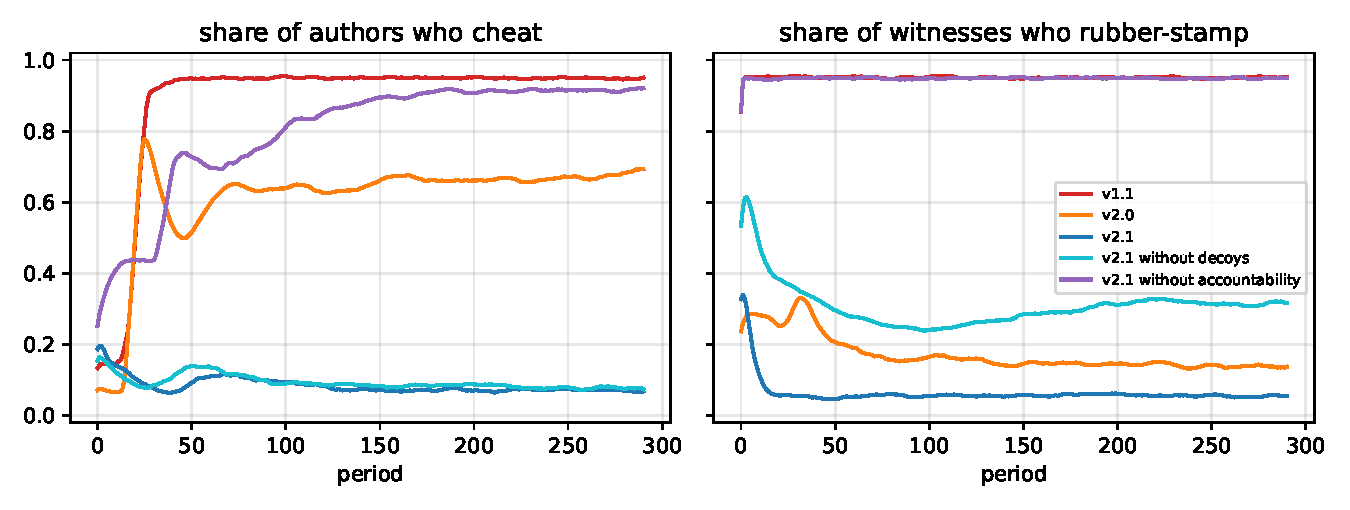
\includegraphics[width=0.95\textwidth]{figures/fig_E6_adaptatifs_en.pdf}
\caption{E6 --- Share of authors who cheat and of witnesses who rubber-stamp
(mean over 50 seeds, 10-period moving average). The floor of about $0.05$
corresponds to $\varepsilon/2$ exploration.}
\label{fig:E6}
\end{figure}

With the v1.1 rules, the system collapses: $95\,\%$ of authors cheat, $95\,\%$
of witnesses rubber-stamp, and $87\,\%$ of frauds are accepted. With v2.0,
witnesses mostly check ($14\,\%$ rubber-stamping), but $68\,\%$ of authors
submit non-conforming signals: saturated at $\tau=1$, they gain nothing by
contributing honestly, and a rejected signal does not make them inactive
(Prop.~\ref{prop:ceiling}). With v2.1, fraud and rubber-stamping stay at the
exploration level ($7.1\,\%$ $[6.3;8.2]$ and $5.5\,\%$ $[5.0;6.0]$) and
$2.1\,\%$ of frauds pass. The two ablations confirm the role of each component:
without decoys, $31\,\%$ of witnesses rubber-stamp and $7.5\,\%$ of frauds pass
(Prop.~\ref{prop:verif}); without witness accountability and author sanction,
the system collapses as in v1.1 ($92\,\%$ fraud, $95\,\%$ rubber-stamping,
$83\,\%$ of frauds accepted). Accountability, seemingly useless with fixed
behaviours (E5), is what prevents collapse when agents adapt.

\subsection{E7 --- Sensitivity}

One factor at a time is varied around the v2.1 configuration (20 members
including 30\,\% colluders and 10\,\% free riders, 100 seeds).
Table~\ref{tab:E7} reports the honest members' final score, the colluders' net
gain, and error rates.

\begin{table}[h]
\centering
\caption{E7 --- Sensitivity of v2.1 (100 seeds per row).}
\label{tab:E7}
\small
\begin{tabular}{lcccc}
\toprule
Variant & honest & colluders' gain & frauds accepted & wrongful rejections \\
\midrule
v2.1 reference & $0.92$ $[0.91;0.93]$ & $-0.44$ & $0.4\,\%$ & $3.7\,\%$ \\
$\sigma_{\text{obs}}=0.05$ & $0.93$ $[0.92;0.94]$ & $-0.44$ & $0.3\,\%$ & $1.2\,\%$ \\
$\sigma_{\text{obs}}=0.20$ & $0.70$ $[0.68;0.72]$ & $-0.45$ & $1.3\,\%$ & $14.1\,\%$ \\
$\sigma_{\text{obs}}=0.20$, $\theta=0.5$ & $0.73$ $[0.71;0.75]$ & $-0.46$ & $5.2\,\%$ & $3.9\,\%$ \\
$\varepsilon_a=0.05$ & $0.91$ $[0.90;0.92]$ & $-0.44$ & $0.4\,\%$ & $3.8\,\%$ \\
$\varepsilon_a=0.05$, no counter-audit & $0.62$ $[0.59;0.65]$ & $-0.45$ & $0.4\,\%$ & $3.8\,\%$ \\
$\varepsilon_a=0.10$ & $0.87$ $[0.86;0.89]$ & $-0.44$ & $0.5\,\%$ & $3.8\,\%$ \\
$\varepsilon_a=0.10$, no counter-audit & $0.36$ $[0.33;0.39]$ & $-0.48$ & $1.1\,\%$ & $3.2\,\%$ \\
$\tau_0=0.3$ & $0.92$ $[0.91;0.93]$ & $-0.26$ & $0.2\,\%$ & $3.8\,\%$ \\
$\tau_0=0.7$ & $0.92$ $[0.91;0.92]$ & $-0.62$ & $0.6\,\%$ & $3.8\,\%$ \\
$n=10$ & $0.92$ $[0.90;0.93]$ & $-0.44$ & $0.3\,\%$ & $3.6\,\%$ \\
$n=40$ & $0.91$ $[0.91;0.92]$ & $-0.44$ & $0.6\,\%$ & $2.4\,\%$ \\
$n=10$, non-adaptive panel & $0.36$ $[0.28;0.45]$ & $-0.44$ & $0.2\,\%$ & $2.1\,\%$ \\
coalition $10\,\%$ & $0.90$ $[0.89;0.91]$ & $-0.44$ & $0.6\,\%$ & $3.7\,\%$ \\
coalition $50\,\%$ & $0.93$ $[0.92;0.94]$ & $-0.46$ & $1.3\,\%$ & $3.7\,\%$ \\
$\theta=0.5$ & $0.92$ $[0.91;0.93]$ & $-0.45$ & $2.3\,\%$ & $1.1\,\%$ \\
$\theta=1$ & $0.88$ $[0.87;0.89]$ & $-0.44$ & $0.0\,\%$ & $12.0\,\%$ \\
$p_a=0.05$ & $0.92$ $[0.91;0.93]$ & $-0.44$ & $0.6\,\%$ & $3.8\,\%$ \\
$p_a=0.30$ & $0.92$ $[0.91;0.93]$ & $-0.44$ & $0.3\,\%$ & $3.7\,\%$ \\
$h=0$ & $0.92$ $[0.91;0.93]$ & $-0.44$ & $0.4\,\%$ & $3.8\,\%$ \\
$h=0.10$ & $0.91$ $[0.90;0.92]$ & $-0.44$ & $0.5\,\%$ & $3.8\,\%$ \\
\bottomrule
\end{tabular}
\end{table}

\begin{figure}[h]
\centering
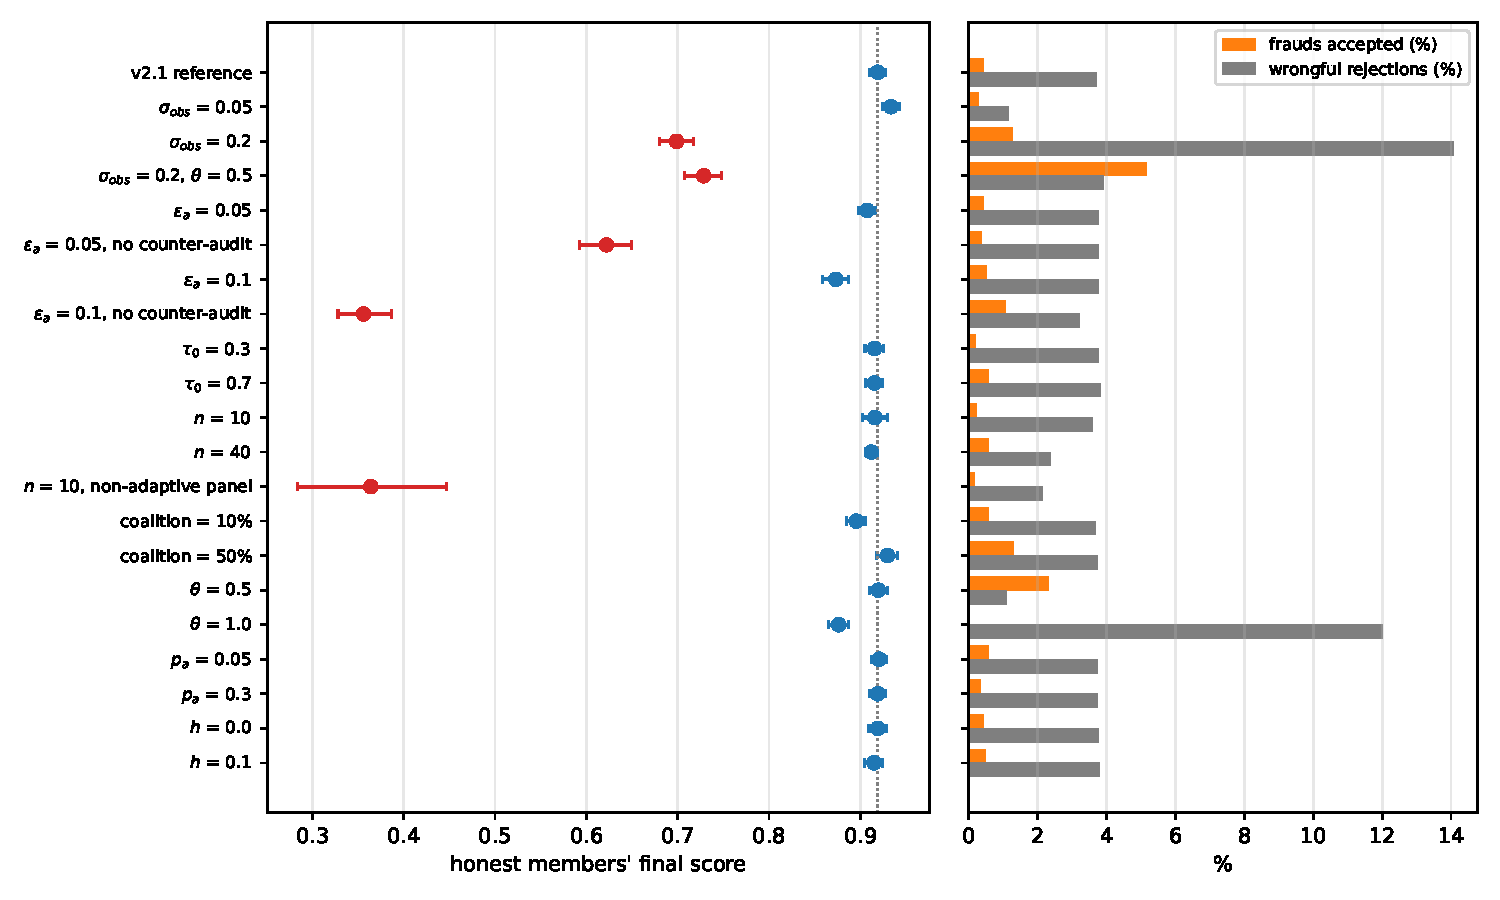
\includegraphics[width=\textwidth]{figures/fig_E7_sensibilite_en.pdf}
\caption{E7 --- Left: honest members' final score per variant (95\,\% CI; red
below $0.8$). Right: frauds accepted and wrongful rejections.}
\label{fig:E7}
\end{figure}

The mechanism (Figure~\ref{fig:E7}) is stable with respect to the initial score, Node size, coalition
size up to 50\,\% ($1.3\,\%$ of frauds accepted), $p_a$ between $0.05$ and
$0.30$, and the decoy rate. Two failure modes, revealed by a first version of
this analysis, led to changes in the model: without counter-audit, a $5\,\%$
audit error brings honest members down to $0.62$ and a $10\,\%$ error to
$0.36$, because every wrongful sanction removes $\phi\tau_w$ from all approvers
and pushes honest members below $\tau_W$; with the counter-audit, they stay at
$0.91$ and $0.87$. In a 10-member Node, a fixed-size panel brings honest
members down to $0.36$ for lack of eligible witnesses; the adaptive panel keeps
them at $0.92$.

The remaining sensitivity concerns witness accuracy. With
$\sigma_{\text{obs}}=0.20$, $14\,\%$ of honest contributions are wrongly
rejected and the honest score drops to $0.70$. Lowering $\theta$ to $0.5$
brings wrongful rejections down to $3.9\,\%$ but lets $5.2\,\%$ of frauds
through, and the honest score only recovers to $0.73$: inaccurate witnesses
themselves approve non-conforming signals and are sanctioned. No tuning
compensates for witnesses unable to judge; this is an applicability condition
of the mechanism (Section~\ref{sec:discussion}).

% ════════════════════════════════════════════════════════════════
\section{Instantiation for tontines}
\label{sec:tontine}
% ════════════════════════════════════════════════════════════════

In a tontine, the main signal --- a contribution payment --- is verifiable from
the payment operator's records. Auditing is therefore exhaustive and nearly free
($p_a=1$, $\varepsilon_a\approx0$), and the witness panel is unnecessary: set
$q=1$ for every payment made on time. Witnesses remain useful for commitments
that cannot be verified automatically (e.g.\ an in-kind contribution). The risk
specific to tontines, a member leaving after receiving the
pot~\cite{anderson2009}, is handled by two rules.

\begin{rulee}[Score-based rotation]
Pot positions are assigned by decreasing score; ties are broken by seniority.
\end{rulee}

\begin{proposition}[Exposure]\label{prop:rotation}
In a tontine of $N$ members with contribution $m$, the member receiving the pot
at position $r$ can, by stopping payments, appropriate at most $(N-r)\,m$.
Under the score-based rotation rule, a member whose score is strictly lower than
all others receives the pot last and has zero exposure.
\end{proposition}
\begin{proof}
At position $r$, the member has paid $rm$ and received $Nm$; $(N-r)m$ remains
to be paid. At position $N$, nothing remains.
\end{proof}

\begin{rulee}[Sponsorship and exclusion]
A newcomer may only join with a sponsor whose score is at least $\tau_W$. They
start at $\tau_p$. During a probation of $P$ periods, each default of the
sponsored member costs $\psi$ to the sponsor. A member whose score reaches 0
after a default is excluded; readmission requires a new sponsor.
\end{rulee}

\begin{proposition}[Defaults before exclusion]\label{prop:sponsor}
Under this rule, a sponsored identity with $C$ accepted contributions in total
commits at most $1+\lfloor(\tau_p+\eta\,C)/\kappa\rfloor$ defaults before
exclusion (excluding witness rewards), and each default during probation costs
$\psi$ to its sponsor. With $\kappa=0.35$ and $\tau_p\le0.35$, an identity that
defaults before any contribution is excluded at its first default.
\end{proposition}
\begin{proof}
The cumulative available score is at most $\tau_p+\eta C$; each default removes
$\kappa$ while the score remains positive, and the default that brings it to 0
triggers exclusion.
\end{proof}

Sponsorship shifts the cost of a new identity --- and hence of Sybil attacks and
of laundering through identity change --- onto an established member, who is
thus incentivised to screen candidates. This is the logic of joint liability in
microcredit~\cite{besley1995,ghatak1999}, and that of guarantors in traditional
tontines. Combined with score-based rotation, it places newcomers at the end of
the rotation, where their exposure is zero, until they have built a track
record.

% ════════════════════════════════════════════════════════════════
\section{Discussion}
\label{sec:discussion}
% ════════════════════════════════════════════════════════════════

\paragraph{What the results establish.} The revised mechanism admits
closed-form conditions confirmed by simulation, and these conditions make it
possible to calibrate it. Each component has an identifiable role: the panel
filters frauds (E3, E5); the inactivity rule makes minority collusion
unprofitable even without audit (Cor.~\ref{cor:noaudit}, E2) and preserves the
incentive at maximal score (Prop.~\ref{prop:ceiling}, E6); witness
accountability and decoys prevent rubber-stamping (Prop.~\ref{prop:verif}, E6);
the audit, backed by a counter-audit, protects against majority coalitions
without penalising honest members (E7).

\paragraph{What witnesses cost.} The panel replaces near-exhaustive auditing
with five votes per signal. It is only worthwhile if a vote costs much less
than an audit.

\paragraph{Applicability condition.} The mechanism assumes witnesses able to
judge conformity with good accuracy (E7). When this is not the case, it is
better to score only automatically verifiable contributions --- which is
precisely the case of tontines (Section~\ref{sec:tontine}), where witnesses
become unnecessary.

\paragraph{Scope.} Previous versions presented \CTP{} as universal. The results
rather show a parameterised framework whose relevant parameters ($\kappa/\eta$,
$\delta/\eta$, $k$, $\theta$, $h$) depend on the nature of contributions, on
witness accuracy and on the cost of an identity; each instantiation must be
calibrated, then evaluated on real data.

% ════════════════════════════════════════════════════════════════
\section{Limitations}
\label{sec:limits}
% ════════════════════════════════════════════════════════════════

\begin{itemize}
  \item \textbf{No real data.} Quality and default distributions and the costs
    $c_h$, $c_v$ are assumed. Appendix~\ref{app:data} describes the required
    data collection protocol.
  \item \textbf{Simple learning.} The E6 agents learn independently; a
    coalition learning jointly, or an adversary trying to recognise decoys, is
    not modelled. Decoy indistinguishability (Assumption~\ref{h:draw}) is a
    design requirement, not a given.
  \item \textbf{Witness accuracy.} The mechanism degrades when witnesses judge
    poorly (E7); measuring this accuracy is a prerequisite for any application
    to non-verifiable contributions.
  \item \textbf{Audit organisation.} The model fixes $p_a$ and
    $\varepsilon_a$ without specifying who audits; outside the case of
    payments, this remains an open question.
  \item \textbf{Utility.} The strategic analysis assumes utility linear in
    score; the actual form of the rights attached to the score is not modelled.
  \item \textbf{Review.} This paper has not been peer reviewed.
\end{itemize}

% ════════════════════════════════════════════════════════════════
\section{Conclusion}
% ════════════════════════════════════════════════════════════════

We reformulated the accountable-witness reputation mechanism of \CTP{} as a
consistent model, derived closed-form conditions for its default tolerance,
collusion resistance, incentives to contribute and to check, and entry cost,
and derived a parameter set from these conditions. Evaluated against baselines,
with adaptive agents and under a sensitivity analysis, the recalibrated
mechanism makes fraud unprofitable where the original rules collapse. Two
failure modes revealed during evaluation were fixed; one applicability
condition --- witness accuracy --- remains. For tontines, the proposed
instantiation uses no witnesses but relies on verifiable payments, score-based
rotation and sponsorship. The next step is empirical: the data collection
described in Appendix~\ref{app:data}.

\paragraph{Reproducibility.} The script
\texttt{simulations-v2.0/ctp\_core\_v2\_experiments.py}
produces all figures, tables and the file \texttt{resultats\_v2.json}, with
fixed seeds.

% ════════════════════════════════════════════════════════════════
\appendix
\section{Erratum for versions v0.1 and v1.1}
\label{app:erratum}
% ════════════════════════════════════════════════════════════════

\begin{enumerate}
  \item \textbf{Anti-collusion condition (Prop.~4.2).} v1.1 claims that
    $\phi\ge3\eta$ suffices for $\tau_w\ge0.3$ and
    $\Prob(\text{detection})\ge0.15$. The stated inequality,
    $\phi>\eta q/(\tau_w\Prob)$, then requires $\phi>22.2\,\eta q$; with
    $\phi=3\eta$ it only holds for $q<0.135$. Moreover, the gain attributed to
    the colluding witness did not exist in the model.
  \item \textbf{No incentive to validate.} Fixed by $R_i$.
  \item \textbf{Audit targeted at $q(s)<q_{\min}$.} Well-rated coalitions were
    never audited. Fixed by uniform auditing.
  \item \textbf{No author sanction.} Fixed by $S_i$.
  \item \textbf{Witness sanction divided by $|\mathcal{W}(s)|$.} Diluted
    accountability. Fixed.
  \item \textbf{Constant consensus factor.} $\min(|\mathcal{W}(s)|/k_j,1)=1$ for
    every accepted signal. Replaced by $|\mathcal{A}(s)|/k$ with $a_k<k$.
  \item \textbf{Convergence (Prop.~3.2).} Undefined $\epsilon$; replaced by
    Proposition~\ref{prop:sat}.
  \item \textbf{Inactivity.} Submitting a signal was enough to stay active,
    which removes the incentive at maximal score (Prop.~\ref{prop:ceiling}, E6).
  \item \textbf{Difficulty index $\rho_j$.} Division by $\tau_{\min}$, which is
    zero as soon as a member reaches 0; the symbol $\rho$ was used for two
    objects. Reformulated in Appendix~\ref{app:extensions}.
  \item \textbf{Simulation-based validation.} With $n=12$, $k=3$, unanimity and
    a single accomplice, the success probability of collusion was zero; the
    code's audit used the true quality, unknown to the protocol; the honest
    score of $1.000$ reflects saturation.
  \item \textbf{Sybil resistance.} Claimed without proof. Replaced by
    Propositions~\ref{prop:sybil} and~\ref{prop:sponsor}.
  \item \textbf{Gas costs.} Unmeasured estimates; removed.
  \item \textbf{References.} Citations in the published v0.1 appeared as
    ``[?]''.
\end{enumerate}

\section{Data collection protocol}
\label{app:data}

Empirical calibration requires, for each tontine followed and each
member-period: the contribution due, the date and amount paid, the pot
position, departures and exclusions, as well as group characteristics (size,
amount, periodicity, age, existence of guarantors).

\paragraph{Sample size.} Estimating a default rate of about $5\,\%$ within
$\pm2$ points with 95\,\% confidence requires about
$1.96^2\times0.05\times0.95/0.02^2\approx456$ independent member-period
observations. Since observations of the same member are correlated, a design
effect of 2 raises this to about 900, e.g.\ three tontines of fifteen members
followed over twenty periods.

\paragraph{Target parameters.} The observed default rate $p_d$ and the
effective tolerance of groups (number of defaults before exclusion) set
$p^\star_d$, hence $\kappa/\eta$ via Corollary~\ref{cor:kappa}; the frequency of
departures after receiving the pot allows testing
Proposition~\ref{prop:rotation}.

\paragraph{Ethics.} Informed consent of members, anonymisation of identities and
amounts before analysis, and reporting results back to the groups.

\section{Out-of-scope extensions}
\label{app:extensions}

v1.1 defined a difficulty index $\rho_j=k_j\bar\tau_j/(k_{\min}\tau_{\min})$,
undefined when $\tau_{\min}=0$. A well-defined form is
$\rho_j=(k_j/k_{\min})\cdot(\varepsilon+\bar\tau_j)/(\varepsilon+\bar\tau_{\mathcal M})$,
where $\bar\tau_{\mathcal M}$ is the mean score across all Nodes and
$\varepsilon>0$. This index, the global score and inter-Node portability are
not analysed here and should not be considered validated.

\section{Notation}

\begin{center}
\small
\begin{tabular}{cl}
\toprule
$\tau_i(t)$ & score of member $i$ \\
$k$, $a_k$, $\theta$ & panel size, required approvals, required fraction \\
$\mathcal{P}(s)$, $\mathcal{A}(s)$ & panel and approvers of signal $s$ \\
$q(s)$, $Q(s)$ & measured quality, true conformity \\
$\eta,\eta_W$ & author gain, witness reward \\
$\kappa,\kappa_s$ & default penalty, author sanction \\
$\delta$, $\phi$ & depreciation, witness accountability \\
$p_a$, $\varepsilon_a$, $h$ & audit probability and error, decoy rate \\
$\tau_W,\tau_0,\tau_p$ & eligibility threshold, founders' and sponsored score \\
$c_h$, $c_v$ & cost of an honest contribution, of a check \\
$p^\star_d, p^\star_a$ & default-tolerance and audit thresholds \\
$\pi$ & panel capture probability \\
$\psi$, $P$ & sponsor penalty, probation length \\
\bottomrule
\end{tabular}
\end{center}

% ════════════════════════════════════════════════════════════════
\begin{thebibliography}{99}
\small

\bibitem{abebe2022}
R.~Abebe, A.~Eck, C.~Ikeokwu and S.~Taggart.
An algorithmic introduction to savings circles.
In \emph{Proc. AAAI Conference on Artificial Intelligence}, 2022.

\bibitem{anderson2009}
S.~Anderson, J.-M. Baland and K.~O. Moene.
Enforcement in informal saving groups.
\emph{Journal of Development Economics}, 90(1):14--23, 2009.

\bibitem{ardener1964}
S.~Ardener.
The comparative study of rotating credit associations.
\emph{Journal of the Royal Anthropological Institute}, 94(2):201--229, 1964.

\bibitem{besley1995}
T.~Besley and S.~Coate.
Group lending, repayment incentives and social collateral.
\emph{Journal of Development Economics}, 46(1):1--18, 1995.

\bibitem{besley1993}
T.~Besley, S.~Coate and G.~Loury.
The economics of rotating savings and credit associations.
\emph{American Economic Review}, 83(4):792--810, 1993.

\bibitem{buterin2021}
V.~Buterin.
Moving beyond coin voting governance.
\url{https://vitalik.ca/general/2021/08/16/voting3.html}, 2021.

\bibitem{cheng2005}
A.~Cheng and E.~Friedman.
Sybilproof reputation mechanisms.
In \emph{Proc. ACM SIGCOMM Workshop on Economics of Peer-to-Peer Systems
(P2PECON)}, pp.~128--132, 2005.

\bibitem{dellarocas2003}
C.~Dellarocas.
The digitization of word of mouth: promise and challenges of online feedback
mechanisms.
\emph{Management Science}, 49(10):1407--1424, 2003.

\bibitem{douceur2002}
J.~R. Douceur.
The Sybil attack.
In \emph{Peer-to-Peer Systems (IPTPS)}, LNCS 2429, pp.~251--260. Springer, 2002.

\bibitem{friedman2001}
E.~J. Friedman and P.~Resnick.
The social cost of cheap pseudonyms.
\emph{Journal of Economics \& Management Strategy}, 10(2):173--199, 2001.

\bibitem{fudenberg1986}
D.~Fudenberg and E.~Maskin.
The folk theorem in repeated games with discounting or with incomplete
information.
\emph{Econometrica}, 54(3):533--554, 1986.

\bibitem{ghatak1999}
M.~Ghatak and T.~W. Guinnane.
The economics of lending with joint liability: theory and practice.
\emph{Journal of Development Economics}, 60(1):195--228, 1999.

\bibitem{handa1999}
S.~Handa and C.~Kirton.
The economics of rotating savings and credit associations: evidence from the
Jamaican `Partner'.
\emph{Journal of Development Economics}, 60(1):173--194, 1999.

\bibitem{hoffman2009}
K.~Hoffman, D.~Zage and C.~Nita-Rotaru.
A survey of attack and defense techniques for reputation systems.
\emph{ACM Computing Surveys}, 42(1):1--31, 2009.

\bibitem{josang2007}
A.~Jøsang, R.~Ismail and C.~Boyd.
A survey of trust and reputation systems for online service provision.
\emph{Decision Support Systems}, 43(2):618--644, 2007.

\bibitem{kamvar2003}
S.~D. Kamvar, M.~T. Schlosser and H.~Garcia-Molina.
The EigenTrust algorithm for reputation management in P2P networks.
In \emph{Proc. 12th International World Wide Web Conference}, pp.~640--651, 2003.

\bibitem{kandori1992}
M.~Kandori.
Social norms and community enforcement.
\emph{Review of Economic Studies}, 59(1):63--80, 1992.

\bibitem{kleros2019}
C.~Lesaege, F.~Ast and W.~George.
Kleros: short paper v1.0.7.
\url{https://kleros.io/assets/whitepaper.pdf}, 2019.

\bibitem{luu2015}
L.~Luu, J.~Teutsch, R.~Kulkarni and P.~Saxena.
Demystifying incentives in the consensus computer.
In \emph{Proc. ACM SIGSAC Conference on Computer and Communications Security
(CCS)}, pp.~706--719, 2015.

\bibitem{marsh1994}
S.~P. Marsh.
\emph{Formalising Trust as a Computational Concept}.
PhD thesis, University of Stirling, 1994.

\bibitem{ostrom1990}
E.~Ostrom.
\emph{Governing the Commons: The Evolution of Institutions for Collective
Action}. Cambridge University Press, 1990.

\bibitem{resnick2000}
P.~Resnick, K.~Kuwabara, R.~Zeckhauser and E.~Friedman.
Reputation systems.
\emph{Communications of the ACM}, 43(12):45--48, 2000.

\bibitem{teutsch2017}
J.~Teutsch and C.~Reitwießner.
A scalable verification solution for blockchains.
arXiv:1908.04756, 2017.

\bibitem{weyl2022}
E.~G. Weyl, P.~Ohlhaver and V.~Buterin.
Decentralized society: finding Web3's soul.
SSRN 4105763, 2022.

\bibitem{xiong2004}
L.~Xiong and L.~Liu.
PeerTrust: supporting reputation-based trust for peer-to-peer electronic
communities.
\emph{IEEE Transactions on Knowledge and Data Engineering}, 16(7):843--857, 2004.

\end{thebibliography}
\end{document}
